
% This LaTeX was auto-generated from an M-file by MATLAB.
% To make changes, update the M-file and republish this document.

\documentclass{article}
\usepackage{graphicx}
\usepackage{color}

\sloppy
\definecolor{lightgray}{gray}{0.5}
\setlength{\parindent}{0pt}

\begin{document}

    
    
\section*{Script to plot an HR diagram}

\begin{par}
Data for the brightest stars, taken from the SDSS web pages at \begin{verbatim}http://cas.sdss.org/dr7/en/proj/advanced/hr/simplehr.asp\end{verbatim}
\end{par} \vspace{1em}
\begin{par}
AH 2010.1.29
\end{par} \vspace{1em}

\subsection*{Contents}

\begin{itemize}
\setlength{\itemsep}{-1ex}
   \item Read in the data from a file called starsTmp.txt
   \item Plot the data
\end{itemize}


\subsection*{Read in the data from a file called starsTmp.txt}

\begin{par}
The file can be created by entering the values into a text-editor window and saving it.
\end{par} \vspace{1em}
\begin{verbatim}
X = importdata('starsTmp.txt',' ');     % read data file
\end{verbatim}


\subsection*{Plot the data}

\begin{verbatim}
clf                         % clear the figure
% First turn the x-axis around: more luminous is more negative
set(axes,'XDir','reverse', 'YDir', 'default')
hold                        % lock plot with with these axis settings
plot(X(:,2), X(:,3), 'o')   % plot data
ylabel('B-V [mag]')         % make labels and title
xlabel('Absolute magnitude [mag]')
title('HR diagram of brightest stars, from the SDSS web pages')
hold                        % release plot
\end{verbatim}

\color{lightgray} \begin{verbatim}Current plot held
Current plot released
\end{verbatim} \color{black}

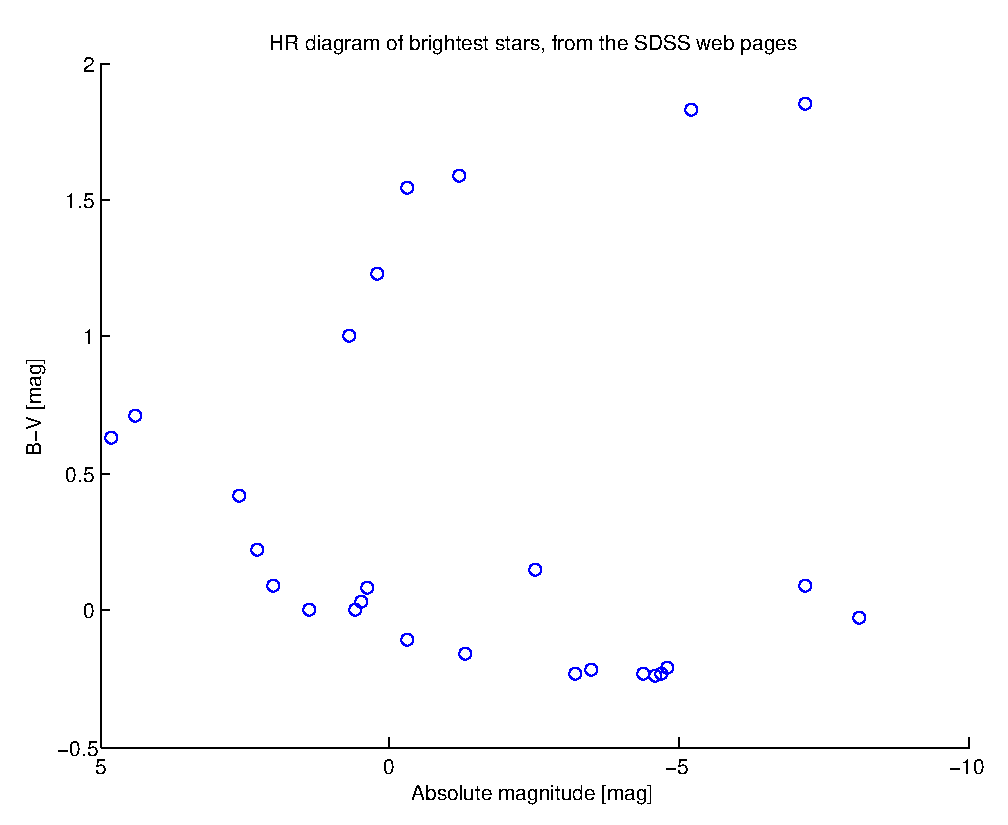
\includegraphics [width=4in]{HR_01.eps}



\end{document}
    
